\newpage
\section{Question 5}
	\newline
	All code used can be found in Appendix A [5].
	\subsection{Part A}
	\newline
	Converted the images into gray scale to use in edge function to find edges of the image. (We have used the image toolbox function edge using ‘sobel’ method. Following was the result. \newline	
	\begin{figure}[position = here]
		\begin{centering}
			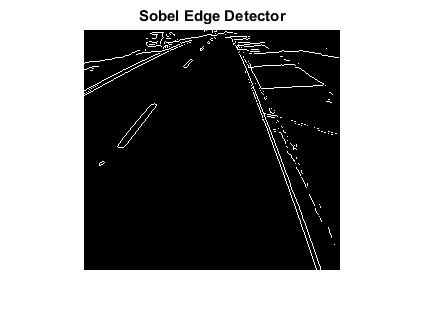
\includegraphics[scale=0.5]{q5_1}\\
			\caption[\textit{RPYAxes}]{Sobel Edge Detector}
		\end{centering}
	\end{figure}
	\newline
	Converted grey image has been used image toolbox function, edge using Canny method to find edges. Following was the result.
	\newline	
	\begin{figure}[position = here]
		\begin{centering}
			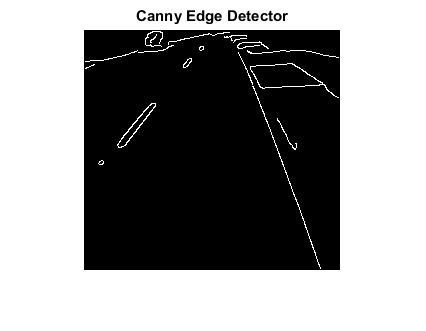
\includegraphics[scale=0.5]{q5_2}\\
			\caption[\textit{RPYAxes}]{Canny Edge Detector}
		\end{centering}
	\end{figure}
	\newline
	
	
	\pagebreak		
	\subsection{Part B}
	\newline
	Converted grey image has been used in image toolbox function, corners using Harris method to find corners. Following was the result.
	\newline	
	\begin{figure}[position = here]
		\begin{centering}
			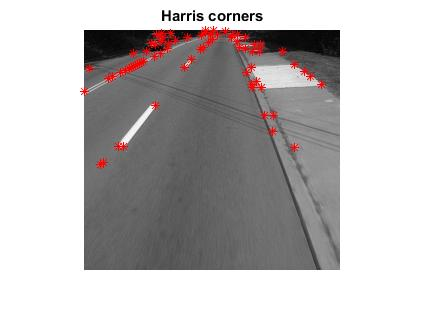
\includegraphics[scale=0.5]{q5_3}\\
			\caption[\textit{RPYAxes}]{Harris Corners}
		\end{centering}
	\end{figure}
	\newline
	
	\subsection{Part C}
	As sift function required input to be a gray image and code is written to read the file from the folder we have saved the converted gray image so that it can open it to use in sift function. Following was the result.
	\newline	
	\begin{figure}[position = here]
		\begin{centering}
			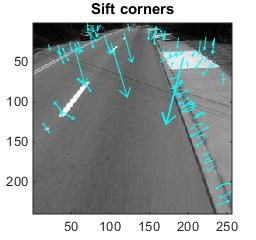
\includegraphics[scale=0.5]{q5_4}\\
			\caption[\textit{RPYAxes}]{Sift Corners}
		\end{centering}
	\end{figure}
	\newline
	\pagebreak
	
	\subsection{Part D}
	\newline
	First I have used given match function to match the given two photos of Whitehouse using sift corners. Following was the result.
	\newline	
	\begin{figure}[position = here]
		\begin{centering}
			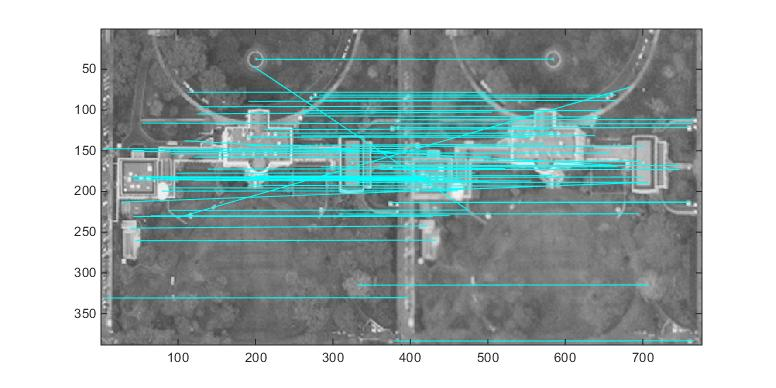
\includegraphics[scale=0.5]{q5_5}\\
			\caption[\textit{RPYAxes}]{Feature Matching 1}
		\end{centering}
	\end{figure}
	\newline
	
	The code we to match features using corners identified using harris corners. We have used feature matching method used in matlab tutorial for matlab image processing toolbox. See Appendix A [5] for the code. This works perfectly with similar (same) images. Result was as follows:
	\newline	
	\begin{figure}[position = here]
		\begin{centering}
			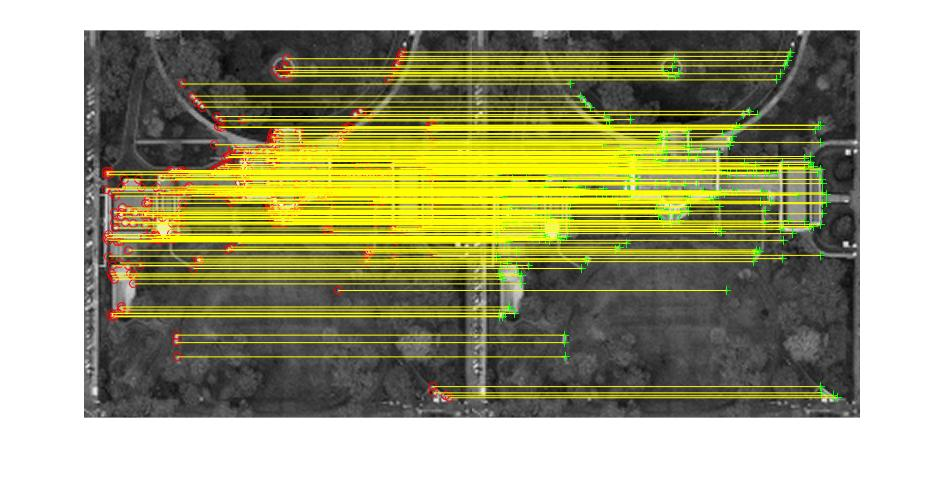
\includegraphics[scale=0.5]{q5_6}\\
			\caption[\textit{RPYAxes}]{Feature Matching 2}
		\end{centering}
	\end{figure}
	\newline
	\newline	
	\begin{figure}[position = here]
		\begin{centering}
			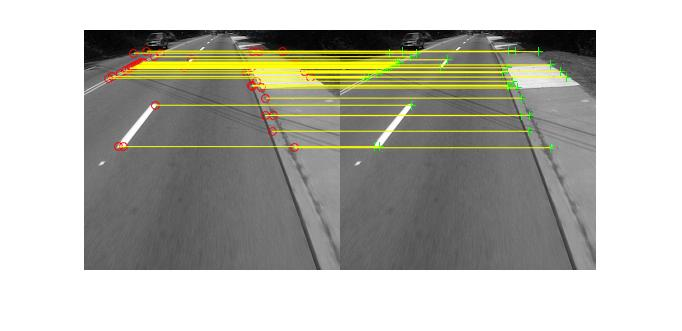
\includegraphics[scale=0.5]{q5_7}\\
			\caption[\textit{RPYAxes}]{Feature Matching 3}
		\end{centering}
	\end{figure}
	\pagebreak
	\newline
	For Slightly different images with similar features result was as follows. For example 1 the result must be improved a lot.
	\newline	
	\begin{figure}[position = here]
		\begin{centering}
			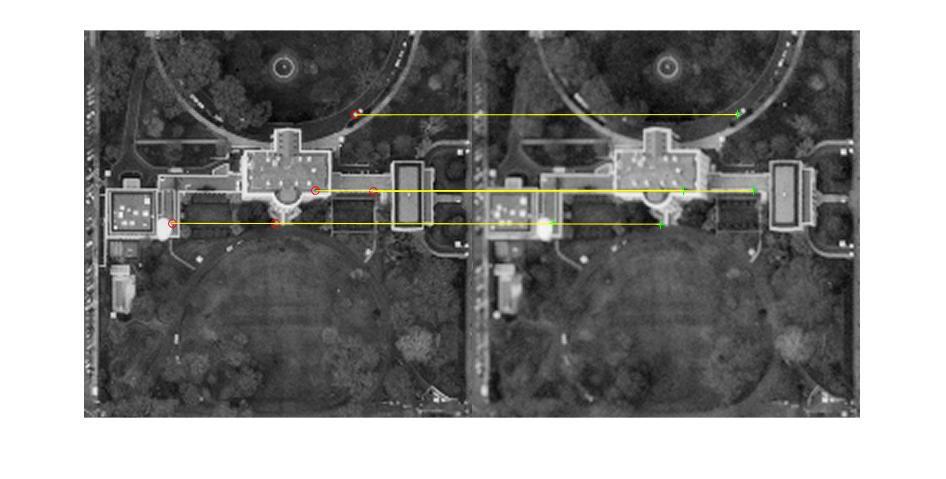
\includegraphics[scale=0.5]{q5_8}\\
			\caption[\textit{RPYAxes}]{Different Matching 1}
		\end{centering}
	\end{figure}
	\newline
	\newline	
	\begin{figure}[position = here]
		\begin{centering}
			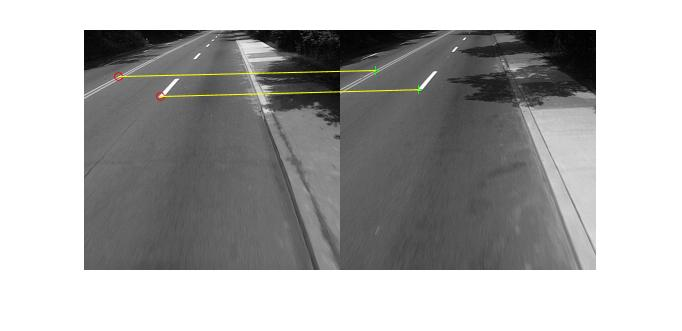
\includegraphics[scale=0.5]{q5_9}\\
			\caption[\textit{RPYAxes}]{Different Matching 2}
		\end{centering}
	\end{figure}
	\newline
		
	\pagebreak
	\subsection*{Code Listing}
	See Appendix A [5] for all code used.
\pagebreak